\documentclass[12pt,a4paper,onecolumn]{article}
\usepackage[utf8]{inputenc}
\usepackage[T1]{fontenc}
\usepackage[french]{babel}
\usepackage{mathrsfs, amsmath}
\usepackage{amsfonts}
\usepackage{amssymb}
\usepackage{amscd}
\usepackage{amsthm}
\usepackage{physics}
\usepackage[left=2.2cm,right=2.2cm,top=2cm,bottom=2cm]{geometry}
\usepackage{textcomp,gensymb} %pour le °C, et textcomp pour éviter les warning
\usepackage{graphicx} %pour les images
\usepackage{caption}
\usepackage{subcaption}
\usepackage[colorlinks=true,
	breaklinks=true,
	citecolor=blue,
	linkcolor=blue,
	urlcolor=blue]{hyperref} % pour insérer des liens
\usepackage{epstopdf} %converting to PDF
\usepackage[export]{adjustbox} %for large figures

\usepackage{array}
\usepackage{dsfont}% indicatrice : \mathds{1}
%\usepackage[dvipsnames]{xcolor}

% -------------------------- Code format ---------------------------------------
\usepackage[numbered,framed]{matlab-prettifier}
\lstset{
  style              = Matlab-editor,
  basicstyle         = \mlttfamily,
  escapechar         = ",
  mlshowsectionrules = true,
}
% ------------------------------------------------------------------------------

% ------------------------- Blbiographie --------------------------------------
% \usepackage[backend=biber, style=science]{biblatex}
% \addbibresource{biblio.bib}
% ------------------------------------------------------------------------------

% ------------------------- Color table ----------------------------------------
\usepackage{multirow}
% \usepackage[table]{xcolor}
% \definecolor{maroon}{cmyk}{0,0.87,0.68,0.32}/
% ------------------------------------------------------------------------------

\setcounter{tocdepth}{4} %Count paragraph
\setcounter{secnumdepth}{4} %Count paragraph
\usepackage{float}

\usepackage{graphicx} % for graphicspath
% \graphicspath{{../images/}}

\usepackage{array,tabularx}
\newcolumntype{L}[1]{>{\raggedright\let\newline\\\arraybackslash\hspace{0pt}}m{#1}}
\newcolumntype{C}[1]{>{\centering\let\newline\\\arraybackslash\hspace{0pt}}m{#1}}
\newcolumntype{R}[1]{>{\raggedleft\let\newline\\\arraybackslash\hspace{0pt}}m{#1}}

\title{TP2 Sub-pixel image processing}
\author{Vincent Matthys}


\renewcommand{\thesubsection}{\alph{subsection}}


\begin{document}
%\maketitle
\begin{tabularx}{0.8\textwidth}{@{} l X r @{} }
{\textsc{Master MVA}} & & \textsc{TP2}\\
\textsc{Sub-pixel image processing} & & {ENS Paris Saclay}\\
%& %M1 Informatique
\end{tabularx}
\vspace{1.5cm}
\begin{center}

\rule[11pt]{5cm}{0.5pt}

\textbf{\LARGE \textsc{Compte-rendu TP2}}
\vspace{0.5cm}\\
Vincent Matthys\\
\rule{5cm}{0.5pt}

\vspace{1.5cm}
\end{center}

\section*{Exercice 4 : Echantillonnage}

\begin{lstlisting}[caption = {Zoom par duplication}]
lambda = 4;
v = u(1:lambda:end, 1:lambda:end);
w = kron(v, ones(lambda));
[ny, nx] = size(u);
imshow([u, w(1:ny, 1:nx)], 'InitialMagnification',100);
\end{lstlisting}
Ce morceau de code permet de simuler un sous-échantillonnage d'un facteur $\lambda$, c'est-à-dire d'effectuer un zoom par duplication. Pour ce faire, on commence par prendre 1 pixel tous les $\lambda$ sur l'image initiale u dans les deux directions. Pour obtenir une image sous-échantillonnée de même taille, on utilise le produit de kronecker avec une matrice de 1, résultant en une image sous-échantillonnée dont les pixels sont dupliqués sur un carré 3x3. On utilise \textit{InitialMagnification} pour avoir un rapport 1 pixel allumé pour 1 élément de la matrice.

\begin{figure}[H]
\begin{center}
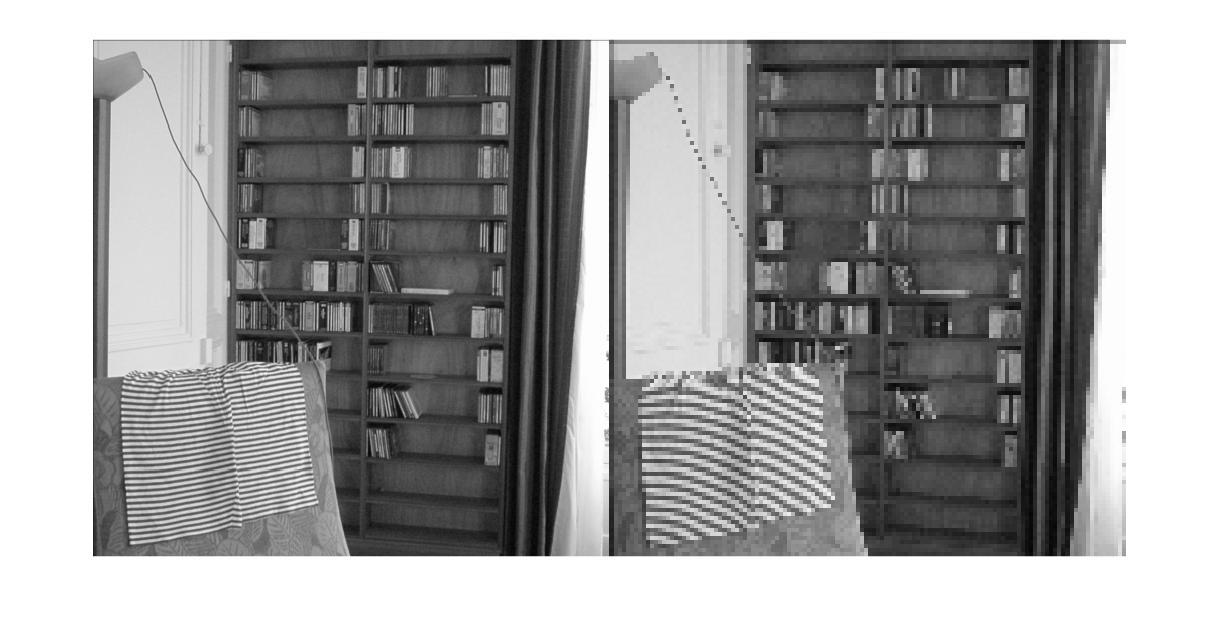
\includegraphics[width = \textwidth]{ex4_1.jpg}
\end{center}
\caption{Image room sous-échantillonnée d'un facteur $\lambda = 4$}
\label{room_l_4}
\end{figure}

Dans la figure \ref{room_l_4} on peut constater les trois types d'aliasing :
\begin{itemize}
	\item repliement spectral, sur le tissu dans la fenêtre $(40, 360)$ à $(220, 450)$.
	\item perte de connexité des structures fines, le long du fil suspendu, par exemple en $(66, 63)$.
	\item crenelage des contours, le long des rideaux, en $(461, 473)$ par exemple.
\end{itemize}
Tous ces phénomènes sont accentués quand on diminue encore l'échantillonnage, c'est-à-dire quand on augmente $\labmda$.

\begin{figure}[H]
\begin{center}
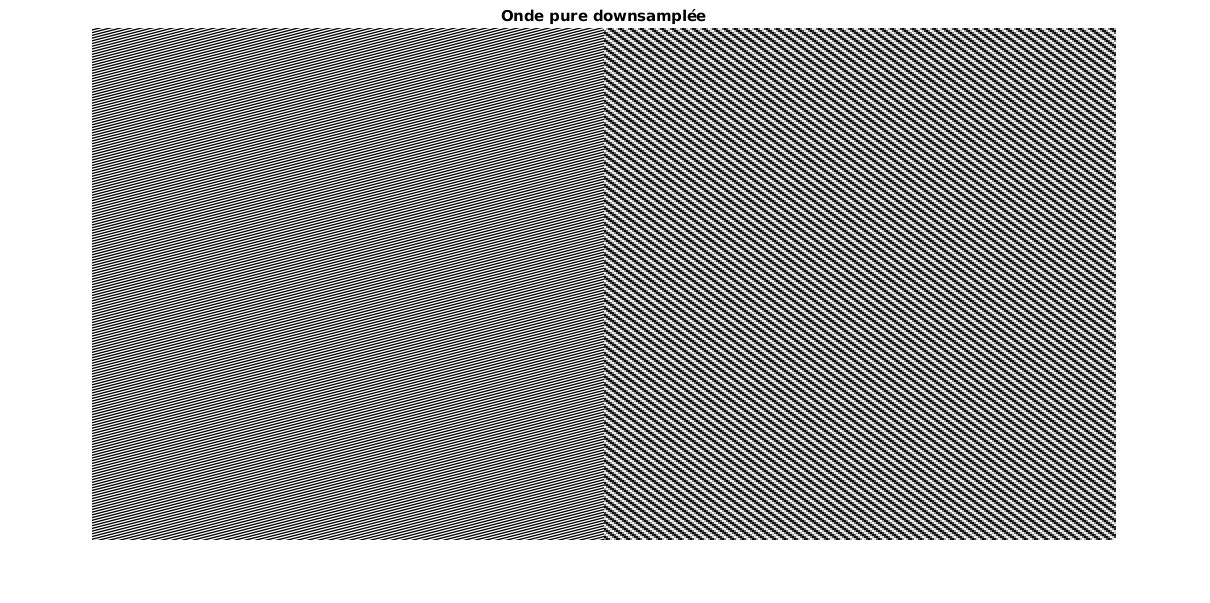
\includegraphics[width = \textwidth]{ex4_onde.jpg}
\end{center}
\caption{Onde initiale et onde sous-échantillonnée d'un facteur 2}
\label{ex4_onde}
\end{figure}

L'onde pure initiale, de fréquence spatiale $(49, 189)$, downsamplée par un facteur deux, produit une onde aussi pure de fréquence spatiale $(49, -67)$, ce qui correspond à un repliement du point en bas à droite sur le carré de Shannon de l'onde initiale, sur la portion en haut à droite du carré de Shannon de l'onde downsamplée. D'où le phénomène observé dans la figure \ref{ex4_onde}, illustration du phénomène d'aliasing dit de repliement spectral.

\paragraph*{Remarques} La FFT de Matlab est cadré de sorte que, pour une image de taille $(N, M)$, sa FFT a pour bornes : $(floor(\frac{N}{2}), N - floor(\frac{N}{2}))$ en x et $(floor(\frac{M}{2}), M - floor(\frac{M}{2}))$ en y.
On notera également que, suite à l'indexation par Matlab, $f(190, 50) = 2$, correspond à ajouter une fréquence spatiale en $(49), 189$.


\section*{Exercice 5}

Dans la figure \ref{ex5_q1}, on constate un phénonène de repliement spectral : les rayures changent de direction après avoir mis au carré l'onde. Cela est en effet attendu. En appelant $\xi_0$ la fréquence spatiale de l'onde pure réelle :
\begin{align*}
\mathscr{F}(u \dotproduct u) &= \mathscr{F}(u) \dotproduct \mathscr{F}(u) \\
& = (\delta_{\xi_0} + \delta_{-\xi_0}) * (\delta_{\xi_0} + \delta_{-\xi_0})\\
& = \delta_{2\xi_0} + 2\delta_{\xi_0 - \xi_0} + \delta_{-2\xi_0}\\
& = \delta_{2\xi_0} +  2\delta_0 + \delta_{-2\xi_0}
\end{align*}
On produit alors une onde pure de fréquence spatiale double, avec une composante continue. A cause de la taille du carré de Shannon, le double de la fréquence initiale ne tombe plus forcément dans le carré initial, ce qui entraîne un repliement de spectre, observé ici avec une fréquence initiale de $(49, 139)$.

\begin{figure}[H]
\begin{center}
	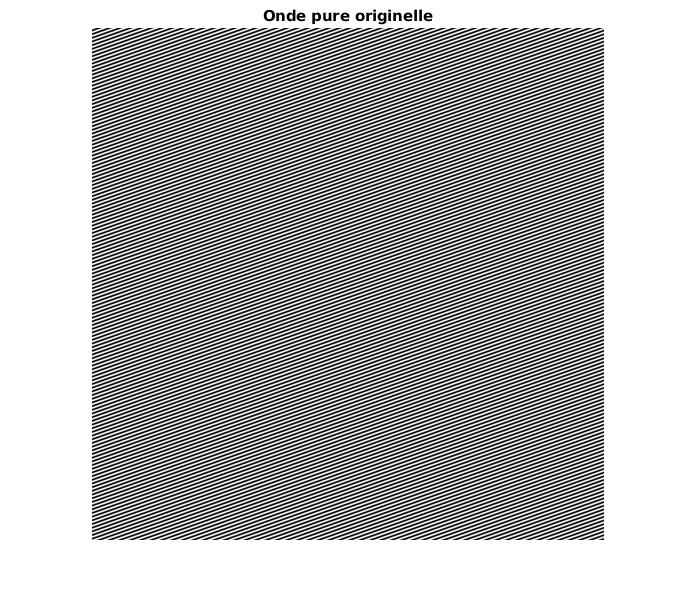
\includegraphics[width = 0.8\textwidth]{ex5_onde.jpg}
	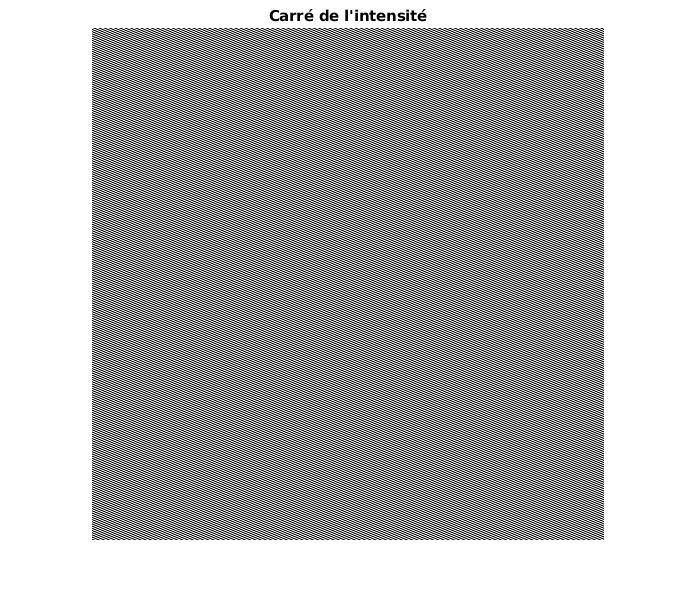
\includegraphics[width = 0.8\textwidth]{ex5_onde_square.jpg}
\end{center}
\caption{Onde initiale, de fréqauence initiale $(49, 139)$ et son carré}
\label{ex5_q1}
\end{figure}

Avec la commande \textit(fftzoom(onde,2)), on peut élargir le support de la transformée de Fourier par 2 dans les 2 directions, permettant à la fréquence double apparaissant après la mise au carré de rester dans la carré de Shannon. On supprime alors le phénomène d'aliasing, et on observe en figure \ref{ex5_q2} une onde de fréquence spatiale de fois plus élevée, mais dans la même direction que l'onde initiale.

\begin{figure}[H]
\begin{center}
	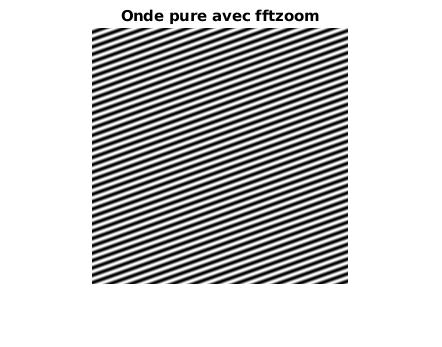
\includegraphics[width = 0.8\textwidth]{ex5_q2_onde.jpg}
	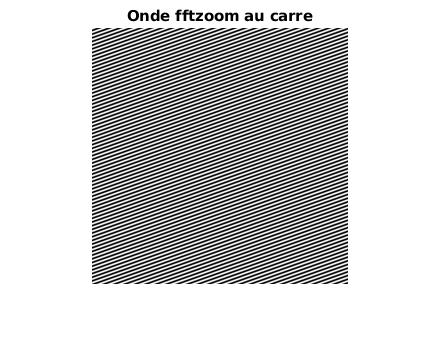
\includegraphics[width = 0.8\textwidth]{ex5_q2_square.jpg}
\end{center}
\caption{Onde renvoyée par \textit{fftzoom} avec un facteur 2, de fréqauence initiale $(49, 139)$ et son carré, toutes deux réduites à la fenêetre $(1, 1)$ jusque $(256, 256)$}
\label{ex5_q2}
\end{figure}

Dans la figure \ref{ex5_q3}, on peut constater qu'on rencontre des phénomènes de repliement de spectre dans le calcul du gradient, notamment au niveau du batiment. Cela, à cause de la manière dont celui-ci est calculè, faisant intervenir la différence au carré sur chaque direction.
\begin{figure}[H]
\begin{center}
	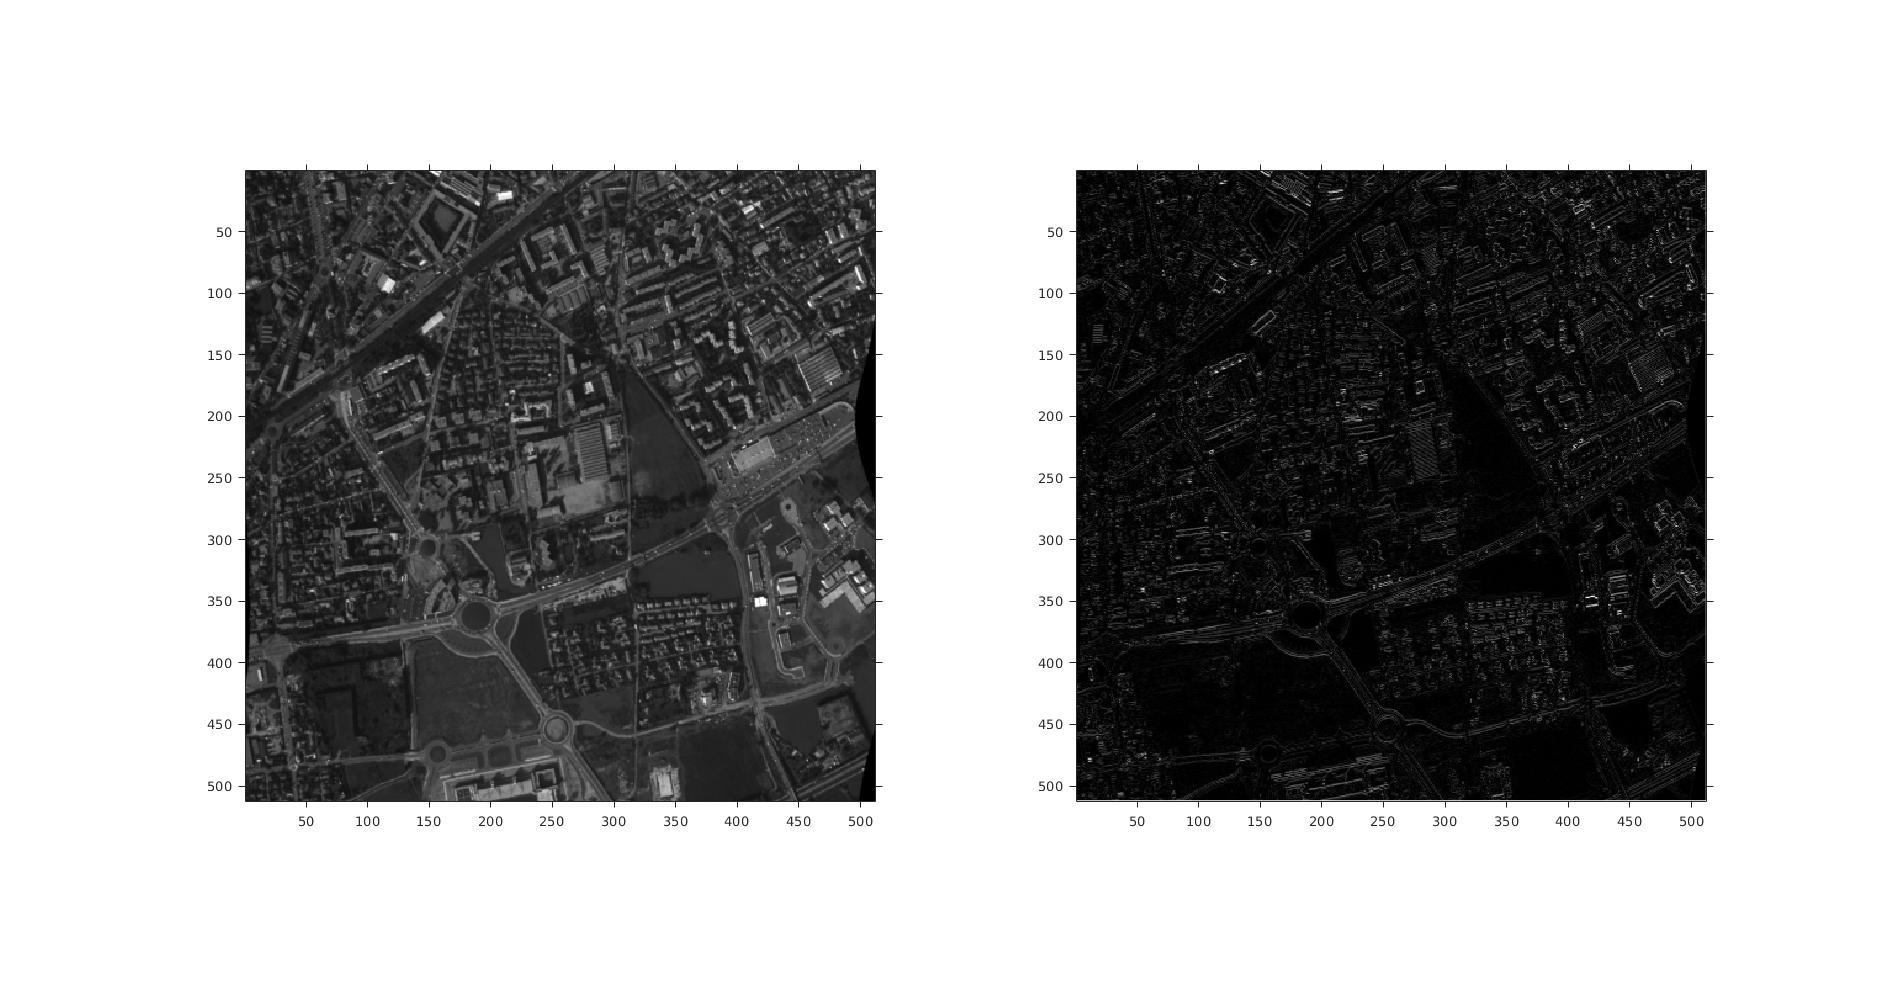
\includegraphics[width = \textwidth]{ex5_q3.jpg}
	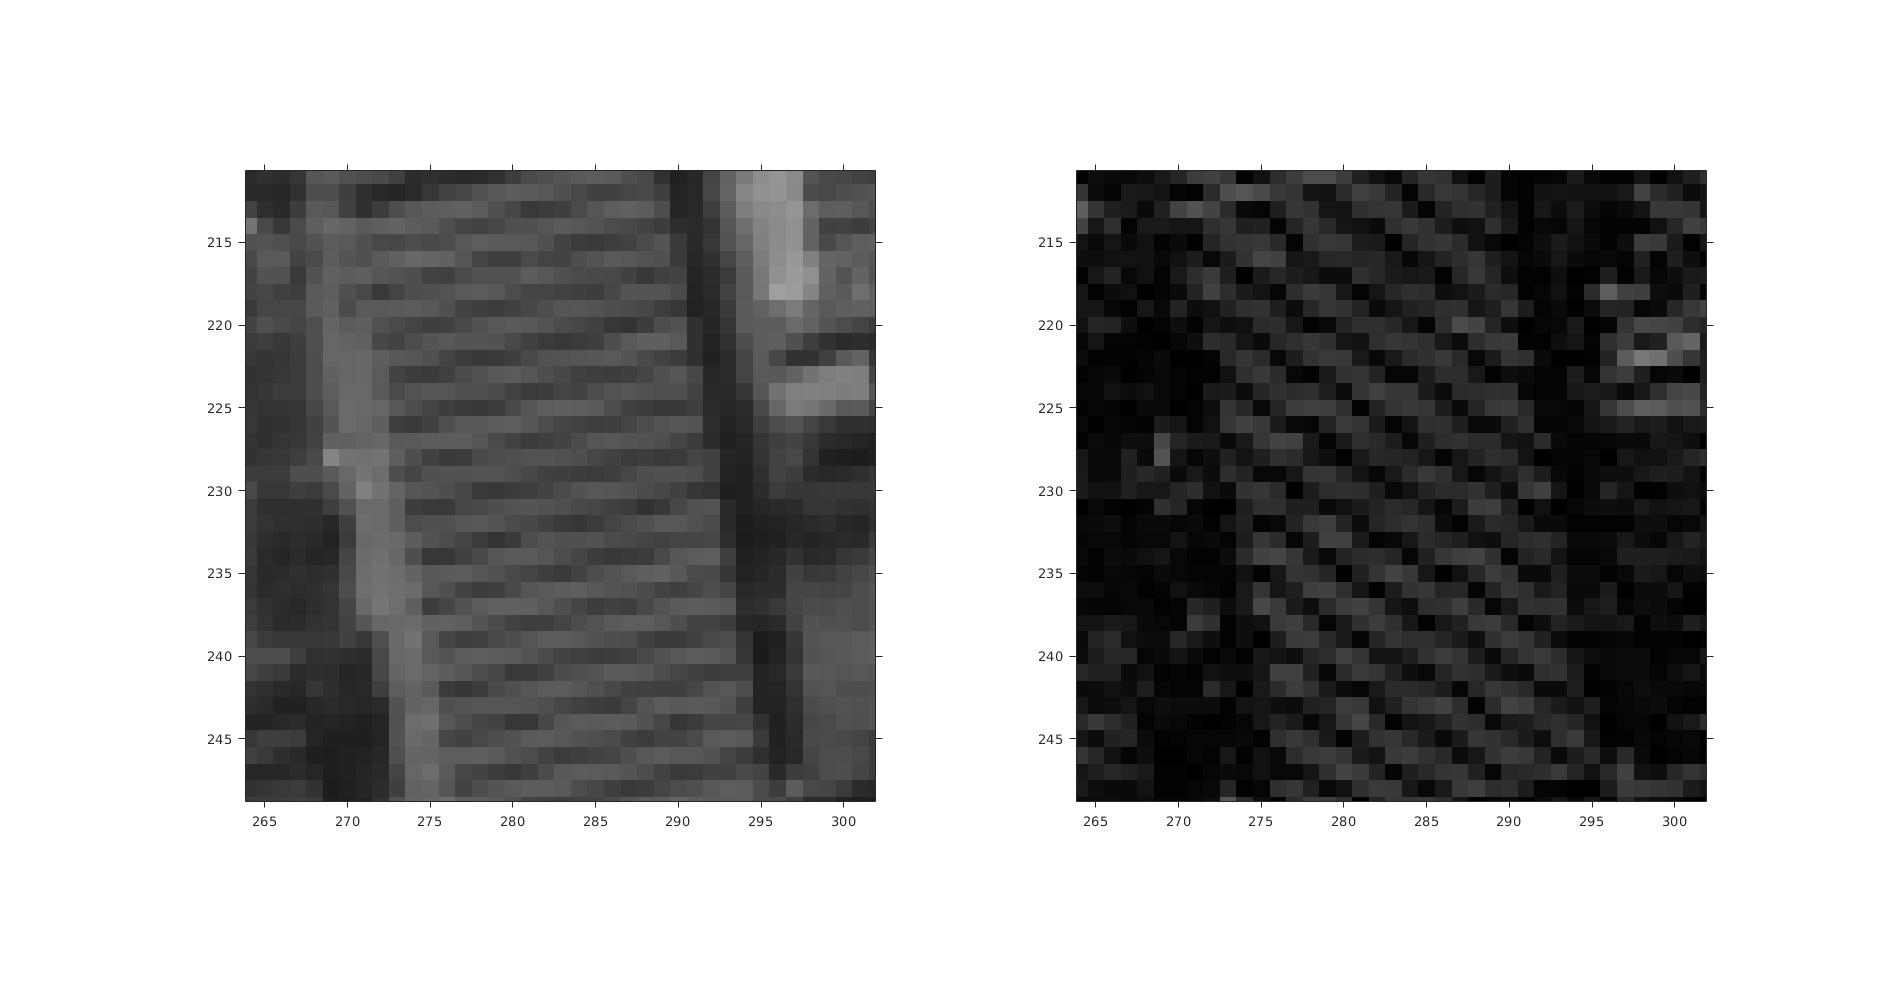
\includegraphics[width = \textwidth]{ex5_q3_building.jpg}
\end{center}
\caption{En haut : image de Nimes. En bas : aggrandissement artificiel de $(265, 210)$ à $(300, 245)$. A gauche : l'image naturelle. A droite : le gradient.}
\label{ex5_q3}
\end{figure}

Pour y remédier, on utilise la même technique que précédemment, avec l'élargissement du spectre de l'image. Le résultat obtenu est présenté en figure
\ref{ex5_q3_sol}. On constate que le phénomène de repliement de spectre a totalemet disparu.

\begin{figure}[H]
\begin{center}
	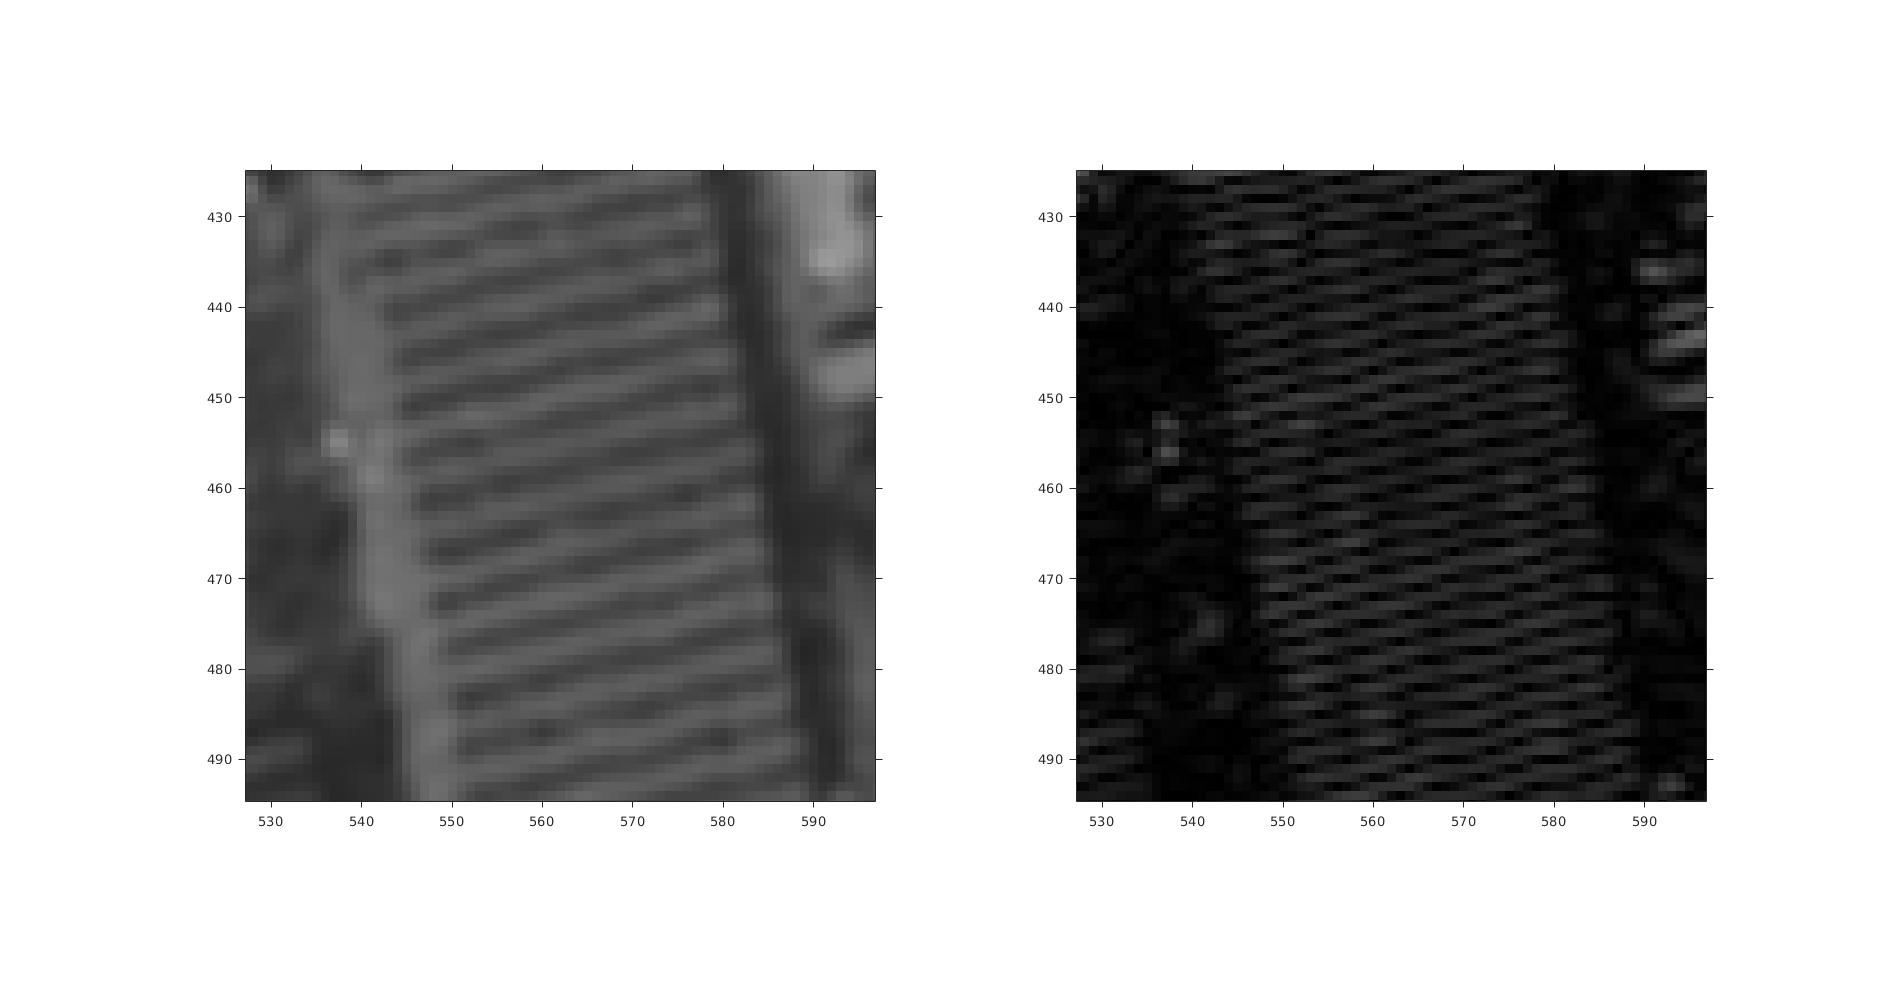
\includegraphics[width = \textwidth]{ex5_q3_solution.jpg}
\end{center}
\caption{Aggrandissement artificiel de $(265, 210)$ à $(300, 245)$ de l'image de Nimes. A gauche : l'image naturelle. A droite : le gradient après élargissement de spectre par \textit{fftzoom}}
\label{ex5_q3_sol}
\end{figure}

\end{document}
